\subsection{Powierzchnia Seiferta}
Zaczniemy od przyjrzenia się powierzchniom.
Niektóre stwierdzenia będziemy przyjmować bez dowodu, by nie rozwodzić się za bardzo nad topologią algebraiczną.

\begin{definition}
    \index{powierzchnia}
    Powierzchnia to dwuwymiarowa rozmaitość topologiczna $M \subseteq \R^3$.
\end{definition}

Rozmaitość to obiekt, który wygląda lokalnie jak przestrzeń euklidesowa: każdy jej punkt $x \in M$ posiada otwarte otoczenie homeomorficzne z~otwartą kulą.
Przykładami powierzchni są sfera, brzeg torusa albo hiperboloida jednopowłokowa.
Istnieje ogólniejsze pojęcie, to jest rozmaitość z~brzegiem: każdy jej punkt posiada otoczenie homeomorficzne z otwartym podzbiorem górnej półpłaszczyzny $\{x \in \C: \mathfrak {Im} \ge 0\}$.
Zwartą powierzchnię bez brzegu nazywamy \emph{domkniętą}.

Powierzchnię nazywamy orientowalną, jeśli nie istnieje na niej zamknięta krzywa, podczas pokonywania której odwraca się kierownica.
Orientowalne są dokładnie te powierzchnie, które nie zawierają w sobie kopii wstęgi Möbiusa.

Najważniejsze dla nas są powierzchnie Seiferta:

\begin{definition}
\index{powierzchnia!Seiferta}
    Powierzchnia Seiferta związana z~węzłem $K$ to spójna,
    orientowanlna powierzchnia zanurzona w~$\R^3$, której brzegiem jest $K$.
\end{definition}

% \begin{example}
% Powierzchnia Seiferta dla trójlistnika:
% \begin{center}
% \begin{tikzpicture}
% [scale=0.1]
%   \clip (-17,-15) rectangle (17,15);
%   \foreach \d in {0,180} {
%       \path[OBSZAR    ,rotate=\d] (-1.25,11.5)
%       .. controls (2,14) and (6,13.5) ..  (10,12)
%       .. controls (23,7) and (15,-20)  .. (3,-13)
%       -- (1.25, -11.5)
%       .. controls (4.5,-8) and (4.5,-4) .. (0,0)
%       .. controls (4,4) and (4.5,5.5) .. (-1.25,11.5);}
%   \path[TIKZ_ARCH] (0,10) .. controls (10,0) and (-10,0) .. (0,-10);
%   \foreach \d in {0,180} {
%   \path[TIKZ_ARCH, rotate=\d] (-1.5,1.5) .. controls (-6,6) and (-3,17) .. (10,12)
%   .. controls (23,7) and (15,-20)  .. (3,-13);}
% \end{tikzpicture}
% \end{center}
% \end{example}

Nie każde uszachowienie diagramu węzła prowadzi do powierzchni Seiferta:
widać to po standardowym diagramie trójlistnika.
Pomimo to...

\begin{proposition}
    \label{seifert_existence}
    Każdy węzeł posiada powierzchnię Seiferta.
\end{proposition}

Powyższe stwiedzenie uzasadnili Pontriagin oraz Frankl w~1930 roku, my jednak podamy bardzo przyjemny i~konstruktywny dowód podany przez Seiferta \cite{seifert35} cztery lata później.
% Frankl, F.; Pontrjagin, L. (1930). "Ein Knotensatz mit Anwendung auf die Dimensionstheorie". Math. Annalen (in German). 102 (1): 785–789. doi:10.1007/BF01782377.

\begin{proof}
    Wybierzmy diagram $D$ dla węzła oraz orientację,
    a~następnie wyprostujmy wszystkie skrzyżowania zgodnie z~ich orientacją:
\begin{comment}
    \[
    \begin{tikzpicture}[scale=0.12, baseline=-3]
        \begin{knot}[clip width=15, end tolerance=1pt,flip crossing/.list={1}]
            \strand[semithick,Latex-] (-5,5) to (5,-5);
            \strand[semithick,-Latex] (-5,-5) to (5,5);
        \end{knot}
    \end{tikzpicture}
    \quad\longrightarrow\quad
        \begin{tikzpicture}[baseline=-0.65ex, scale=0.12]
        \useasboundingbox (-5, -6) rectangle (5, 6);
        \draw[semithick,-Latex] (-4, -5) to [out=45, in=-45] (-4, 5);
        \draw[semithick,-Latex] (4, -5) to [out=135, in=-135] (4, 5);
        \end{tikzpicture}
        \quad\longleftarrow\quad
    \begin{tikzpicture}[scale=0.12, baseline=-3]
        \begin{knot}[clip width=15, end tolerance=1pt]
            \strand[semithick,Latex-] (-5,5) to (5,-5);
            \strand[semithick,-Latex] (-5,-5) to (5,5);
        \end{knot}
    \end{tikzpicture}
    \]
\end{comment}

    Otrzymany diagram składa się teraz z~pewnej liczby zamkniętych krzywych,
    zwanych okręgami Seiferta, które wypełniamy do dysków.
    Tam, gdzie jeden okrąg leżał wewnątrz drugiego, podnosimy wewnętrzny nad zewnętrzny.
    Przy każdym skrzyżowaniu pierwotnego diagramu doklejamy skręcony pasek do obydwu dysków.

    \begin{figure}[H]
        \centering
        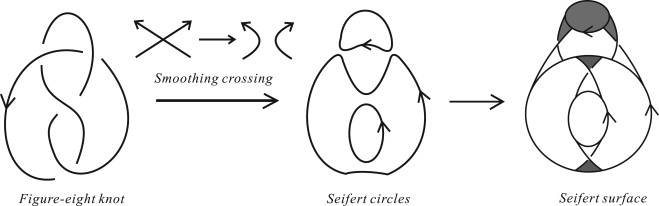
\includegraphics[width=0.75\textwidth]{../data/seifert-algorithm.jpg}
        \caption[Smthing]{Kolejne kroki algorytmu Seiferta}
    \end{figure}

    Dyski są dwustronne, więc ich górnej stronie przypisujemy znak $+$,
    jeśli tylko brzeg jest zorientowany dodatnio i~$-$ w~przeciwnym razie.
\end{proof}

Powierzchnia Seiferta dziedziczy orientację po węźle.
Nawet niewinne odwrócenie jednego z ogniw splotu potrafi istotnie zmienić jego powierzchnię, dlatego potrzebna jest ostrożność!
Zanim przejdziemy do zdefiniowania macierzy Seiferta, potrzebować będziemy krótkiego skoku w bok -- zrozumieć bardzo geometryczny niezmiennik węzłów, genus.

\index{węzeł!rozwłókniony}
Wspomnijmy jeszcze krótko o~specjalnym rodzaju węzłów i splotów.

\begin{definition}
    Niech $L \subseteq S^3$ będzie splotem.
    Jeśli istnieje rodzina $F_t$ powierzchni Seiferta dla splotu $K$ sparametryzowana przez $t \in S^1$ taka, że $F_t \cap F_s = K$ dla $t \neq s$, to splot $K$ nazywamy rozwłóknionym albo włóknistym(z~angielskiego \emph{fibered}.)
\end{definition}

Dawniej nazywano je splotami Neuwirtha, gdyż ten pokazał w~swojej pracy dyplomowej z~1959 roku, że można je scharakteryzować jako sploty, których komutant grupy podstawowej jest skończenie generowany, lub równoważnie, wolny.
Niewęzeł, trójlistnik, ósemka i~splot Hopfa są rozwłóknione, podobnie węzły torusowe.

\begin{proposition}
    Pierwszy i~ostatni współczynnik wielomianu Alexandera węzła rozwłóknionego to $\pm 1$.
\end{proposition}

Kryterium to jest wystarczające dla węzłów pierwszych o co najwyżej 10 skrzyżowaniach oraz alternujących, ale znany jest przykład niewłóknistego węzła o 21 skrzyżowaniach, którego wielomian Alexandera ma postać $t^4 - t^3 + t^2 - t +1$.

Wielomianem węzła skręconego (patrz \ref{twist_knots}) z~$q$ półskrętami jest
\begin{equation}
    \alexander_q(t) = q \cdot \left(t + \frac 1 t\right)  - (2q+1),
\end{equation}
więc poza przypadkiem $q = 1$ nie jest on rozwłókniony.
W szczególności węzeł $6_2$ nie jest rozwłókniony.

\begin{proposition}
    Rodzina węzłów rozwłóknionych jest zamknięta na branie sum spójnych.
\end{proposition}

Rolfsen podaje to jako ćwiczenie w swojej książce.

% Węzeł jest rozwłókniony dokładnie wtedy, gdy stanowi grzbiet pewnego 'open book decomposition' $S^3$.
